\documentclass[conference,10pt,compsocconf]{IEEEtran}

% *** CITATION PACKAGES ***
%
\usepackage{cite}
% cite.sty was written by Donald Arseneau
% V1.6 and later of IEEEtran pre-defines the format of the cite.sty package
% \cite{} output to follow that of IEEE. Loading the cite package will
% result in citation numbers being automatically sorted and properly
% "compressed/ranged". e.g., [1], [9], [2], [7], [5], [6] without using
% cite.sty will become [1], [2], [5]--[7], [9] using cite.sty. cite.sty's
% \cite will automatically add leading space, if needed. Use cite.sty's
% noadjust option (cite.sty V3.8 and later) if you want to turn this off.
% cite.sty is already installed on most LaTeX systems. Be sure and use
% version 4.0 (2003-05-27) and later if using hyperref.sty. cite.sty does
% not currently provide for hyperlinked citations.
% The latest version can be obtained at:
% http://www.ctan.org/tex-archive/macros/latex/contrib/cite/
% The documentation is contained in the cite.sty file itself.
%
\usepackage{setspace}
\usepackage{wrapfig}
\usepackage{color}
\usepackage{balance}

%\usepackage[pdftex]{graphicx}
\usepackage{graphicx}
% declare the path(s) where your graphic files are
\graphicspath{{./}{./figs}}
% and their extensions so you won't have to specify these with
% every instance of \includegraphics
\DeclareGraphicsExtensions{.pdf,.jpeg,.png}

% *** SUBFIGURE PACKAGES ***
\usepackage[tight,footnotesize]{subfigure}
% \usepackage{subfigure}
% subfigure.sty was written by Steven Douglas Cochran. This package makes it
% easy to put subfigures in your figures. e.g., "Figure 1a and 1b". For IEEE
% work, it is a good idea to load it with the tight package option to reduce
% the amount of white space around the subfigures. subfigure.sty is already
% installed on most LaTeX systems. The latest version and documentation can
% be obtained at:
% http://www.ctan.org/tex-archive/obsolete/macros/latex/contrib/subfigure/
% subfigure.sty has been superceeded by subfig.sty.

%\usepackage[caption=false]{caption}
%\usepackage[font=footnotesize]{subfig}
% subfig.sty, also written by Steven Douglas Cochran, is the modern
% replacement for subfigure.sty. However, subfig.sty requires and
% automatically loads Axel Sommerfeldt's caption.sty which will override
% IEEEtran.cls handling of captions and this will result in nonIEEE style
% figure/table captions. To prevent this problem, be sure and preload
% caption.sty with its "caption=false" package option. This is will preserve
% IEEEtran.cls handing of captions. Version 1.3 (2005/06/28) and later
% (recommended due to many improvements over 1.2) of subfig.sty supports
% the caption=false option directly:
%\usepackage[caption=false,font=footnotesize]{subfig}
%
% The latest version and documentation can be obtained at:
% http://www.ctan.org/tex-archive/macros/latex/contrib/subfig/
% The latest version and documentation of caption.sty can be obtained at:
% http://www.ctan.org/tex-archive/macros/latex/contrib/caption/

% *** PDF, URL AND HYPERLINK PACKAGES ***
%
\usepackage{url}
% url.sty was written by Donald Arseneau. It provides better support for
% handling and breaking URLs. url.sty is already installed on most LaTeX
% systems. The latest version can be obtained at:
% http://www.ctan.org/tex-archive/macros/latex/contrib/misc/
% Read the url.sty source comments for usage information. Basically,
% \url{my_url_here}.

% *** Do not adjust lengths that control margins, column widths, etc. ***
% *** Do not use packages that alter fonts (such as pslatex).         ***
% There should be no need to do such things with IEEEtran.cls V1.6 and later.
% (Unless specifically asked to do so by the journal or conference you plan
% to submit to, of course. )

\begin{document}
\title{Optimizing Application Performance on a Burst Buffer using
Holistic I/O Characterization}

\maketitle

\begin{abstract}

\textcolor{red}{TODO: this abstract is already out of sync, likely to have
more emphasis on burst buffer at least.}

A variety of instrumentation and analysis tools have been utilized to
great effect to help understand and optimize components such as disk
arrays, file servers, libraries, and applications.  However, these
tools operate in isolation with a limited view of the system as a whole.
An integrated, holistic approach to I/O characterization is needed on
today's increasingly complex systems in order to fully understand
the interactions between components.  These complex interactions are what 
ultimately dictate overall scientific productivity in practice.

In this work we explore a case study in holistic I/O characterization
using an exemplar scientific computing application [description(s?)] on
Cori [description].  Our case study brings together characterization from
X,Y,Z to illustrate how [application performance?  system performance?]
could be improved via integrated holistic I/O characterization.
We make THING A go B \% faster for a meaningful workload.  We evaluate
our instrumentation methods and find that this approach is not only
highly valuable for case studies, but is also entirely feasible for
ongoing 24/7 production deployment without perturbing applications [some
empirical backup].  Finally, we propose a set of recommendations for
how this methodology can be automated in the future.

\end{abstract}

\section{Introduction}

\emph{From Rob}: I think a component of the story is that when we approach these problems, there are a few challenges:
\begin{enumerate}
\item increasing number of interoperating components (in this case, additional
BB and DVS and so forth)
\item different components have different "views" on I/O, different levels of
monitoring, some of which aren't practical in production
\item no current framework for integration, lots of expert knowledge to
construct the story of what happened and how to fix.
\end{enumerate}
Cite something to get bibtex working for now~\cite{carns200924}.

\section{Background}

\subsection{Platform}

We used Cori, NERSC's Cray XC40 featuring 144 burst buffer nodes sprayed
across the dragonfly network.

\subsection{Instrumentation sources}

\section{Case studies}

\subsection{VPIC}

Description: VPIC-IO kernel; uses HDF and collective I/O (and thus collective
buffering) for bursts of write activity.  Right now we have 2K and 16K core
examples, with and without burst buffer.  When burst buffer is used it is 20
nodes on 2K runs and 87 nodes on 16K runs.

Questions:
\begin{itemize}
\item Are the collective buffering settings appropriate for BB?
    \begin{itemize}
    \item Is collective buffering even appropriate?
    \item Are we using the right number of aggregators in the right place?
    \end{itemize}
\item Why does performance change radically with only a slight change in the
number of BB nodes?
    \begin{itemize}
    \item Related to collective buffering (see above) or some other problem?
    \end{itemize}
\end{itemize}

\subsection{BLAST}

Description: benchmark representing BLAST application.  Many small read
operations, no coordination across processes.

Questions:
\begin{itemize}
\item Does this workload show more or less benefit than VPIC from using BB?
\item Does it make more sense to stage-in private copies of DB at every
node, or to stage-in a single shared DB?
    \begin{itemize}
    \item Both from app and system perspective.
    \end{itemize}
\end{itemize}

\subsection{Staging}

Description: staging data in and out of burst buffers for use by arbitrary
applications.

\begin{itemize}
\item How long does it take to stage in or stage out data?
    \begin{itemize}
    \item How does this compare to explicit copying?
    \end{itemize}
\item On stage out, is it using appropriate Lustre striping?
\item On stage in or stage out, is it using appropriate access sizes?
    \begin{itemize}
    \item In particular, does it make workload for Lustre look better than if
    application had issued small writes (for example) directly?
    \end{itemize}
\item Can applications use Datawarp API to asynchronously push out previous
checkpoints while computing next interval?
    \begin{itemize}
    \item Previous experiments indicate that this isn't as asynchronous as
    hoped for
    \end{itemize}
\end{itemize}

\section{Characterization techniques}

Description: What did we learn about our characterization methodology?  Is it
viable to leave this continuously and provide data processing tools to
automate what we showed in this paper?

What enhancements do we recomment (some of which we may have already done)
\begin{itemize}
\item Darshan: be able to understand aggregator behavior even when shared
file records are reduced to one record
\item Darshan: collect Lustre layout information to enhance correlation
\item DVS: automatic prolog/epilog to collect counters
    \begin{itemize}
    \item can we coordinate this with the Darshan 3.1 epilog scripts?
    \end{itemize}
\item DVS: time series sampling, as in procmon?
\item DVS: vendor could help us out by counting bytes transferred
\item DVS: collect list of BB nodes that were used
\end{itemize}

\section{SCRATCH: visualization example}

It would be nice if we had a default figure to show the holistic view at a
high level.  Something that we could just generate from a script given a set
of logs.  It won't attempt to capture everything, but just show high level
relationship between our instrumentation points.  Something that we can
quickly show for each application use case example.  We then use detailed
one-off graphs to dig into particular relevant aspects of the case study.

\begin{figure}
\centering
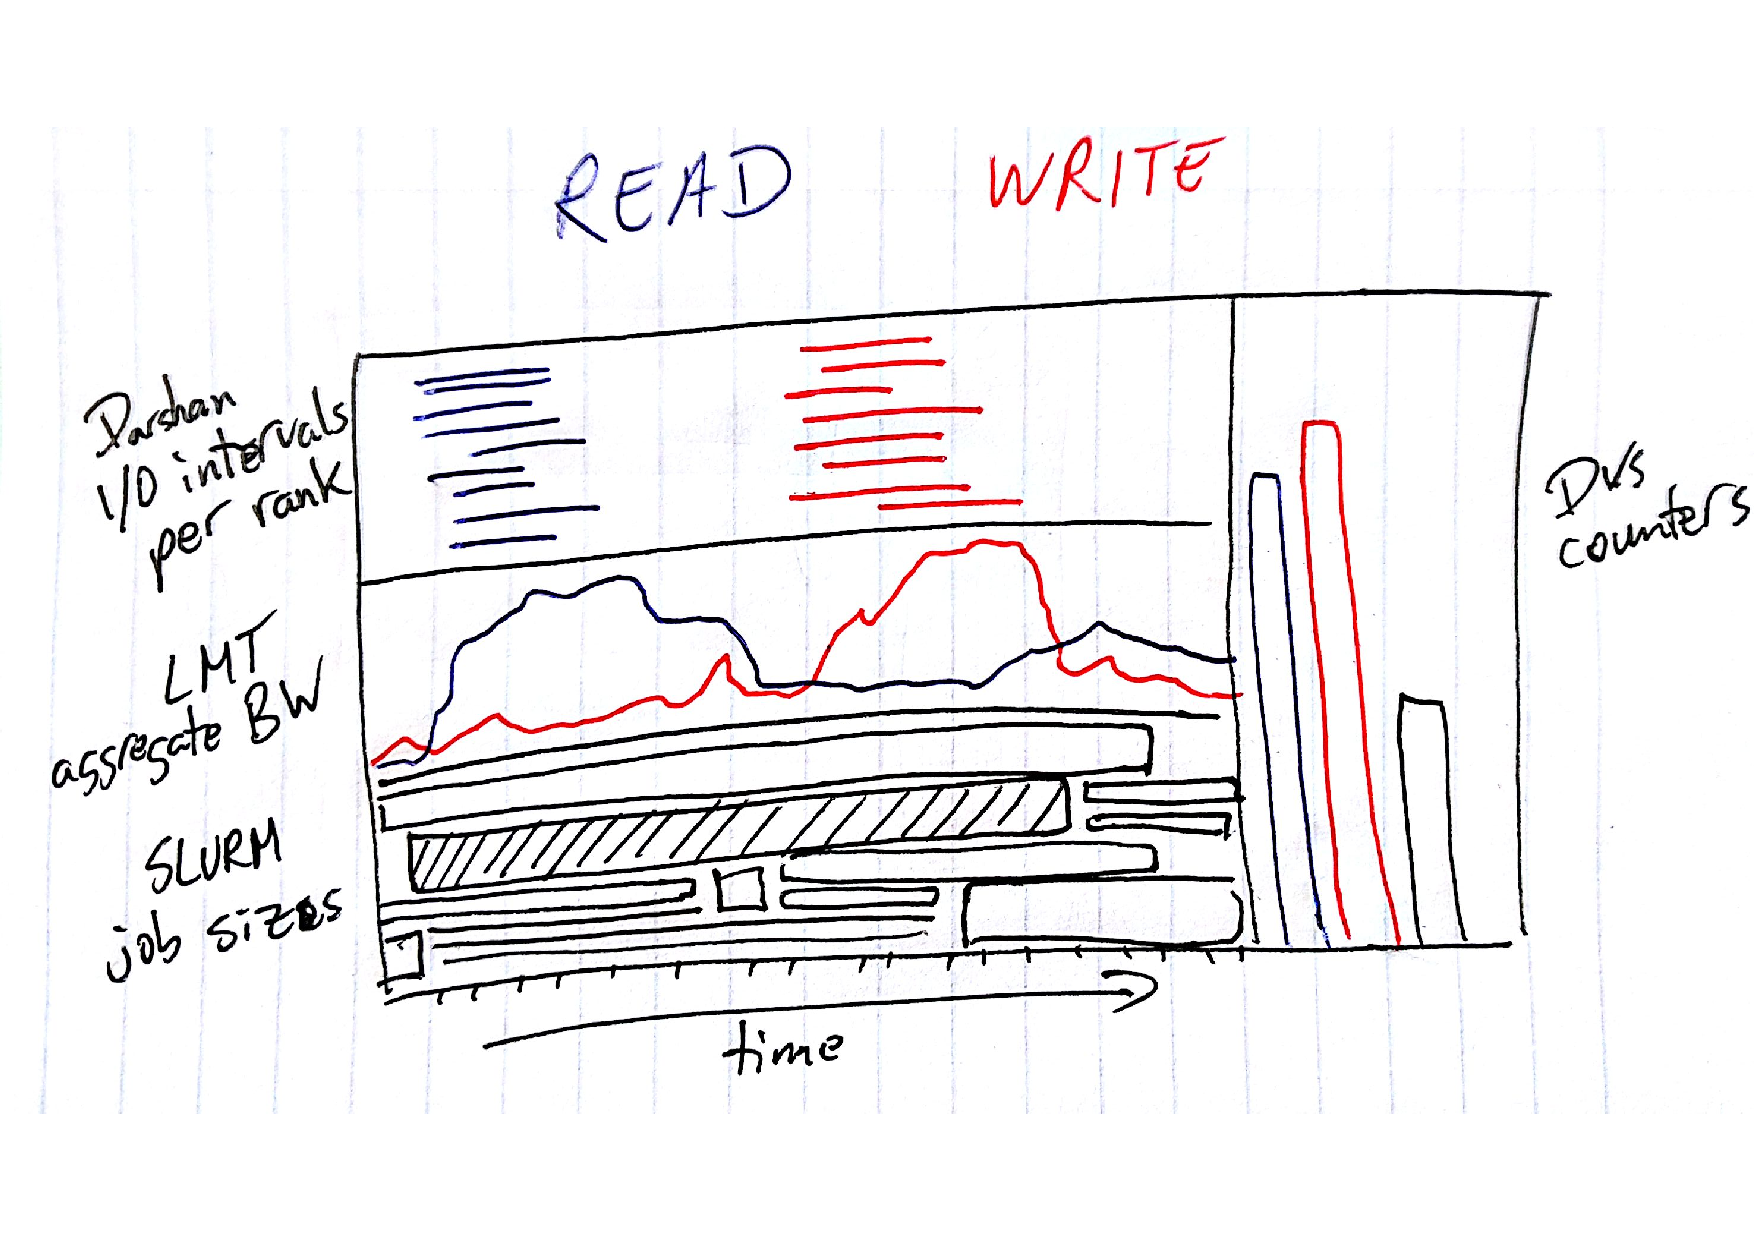
\includegraphics[width=0.5\textwidth]{figs/holio-fig-sketch.pdf}
\caption{Proposal for a default ``high-level'' view of a job, encompassing
multiple data sources.  We would want a perl/python script that can produce
this quickly from a set of logs.  Would be used for overview or comparison of
runs before digging into custom analysis.}
\label{fig:holio-fig-sketch}
\end{figure}

Figure~\ref{fig:holio-fig-sketch} is a sketch of an example.  We 3 things
that can be shown in a stack with a shared x axis for time.  The top one is
the intervals of I/O activity for each rank according to Darshan (we probably
need to run Darshan in the mode that disables reduction to make something
interesting here on a consistent basis).  The middle one is just the
aggregate bandwidth (read and write) reported by LMT over the same time
period.  The bottom one shows each job that was running on the system during
that time interval.  Each job is a rectangle, with height indicating number
of nodes the job used, length indicating duration of job.  So we can see if
bigger jobs were overlapping, for example.

The DVS data is not time series at present, so we just show it on the right
side as a set of histograms (not sure which ones) showing how much activity
happened on the burst buffer in the job.

Comments?  Is this something we can write a script to generate right now?

We could also put an annotation somewhere on there that indicates what
percentage of the LMT traffic is accounted for by Darshan (the DVS counters
are zero, at least).  For a rough idea of contention: ``45\% of Lustre read
traffic and 82\% of Lustre write traffic during this job run came from this
job.''

\section{SCRATCH: temporary notes}

\begin{itemize}
\item Breakdown of raw LMT data:
    \begin{itemize}
    \item For every 5s interval:
        \begin{itemize}
        \item For each OST: bytes read, bytes written, CPU \%
        \item For each MDS: frequency counts of a bunch of ops (opens, close, getattr, ...)
        \end{itemize}
    \item Contrast with Darshan data related to time stamps:
        \begin{itemize}
        \item Darshan only stores absolute time of job start and end times
        \item Darshan stores a few relative timestamps of first and last open/read/write/close ops
        \end{itemize}
    \item Shane has some scripts for post-processing LMT data into a format that is more easily
          graphable, and made the following observations:
        \begin{itemize}
        \item CPU PCT is always 0 -- If we want to look at this metric, Glenn will need to find this
              data in another LMT table
        \item Some missing intervals in LMT data -- Glenn: LMT uses UDP and can drop packets, so
              keep this in mind when analyzing this data
        \end{itemize}
    \item Glenn: still need to grab LMT data for \textbf{after} the BB runs, since this is whe data
          is flushed to Lustre
    \end{itemize}
\item Incorporation of Lustre module into Darshan
    \begin{itemize}
    \item All: a Lustre module would be pretty useful...
    \item Shane has stubbed out Lustre module implementation he has shared with Glenn
        \begin{itemize}
        \item Need to determine lowest overhead way of getting data: /proc or liblustre API?
        \item Grab anything else besides: stripe params and OSTs associated with each file?
        \item If enabled, every file opened at the POSIX layer will be handed to the Lustre
              module to obtain Lustre data
        \item Glenn: stripe params and OST mappings are immutable, so these data records
              only need to be set once per file
        \end{itemize}
    \end{itemize}
\item Initial observations of VPIC-IO runs:
    \begin{itemize}
    \item Glenn: every proc is opening the file, though only 1/3 are writing. Could the
          low BB performance be due to the large metadata workload?
        \begin{itemize}
        \item Phil: compare ratio of I/O to metadata time for the Lustre runs and the BB
              runs to confirm
        \item Phil: MPI-IO hints can be used to force only aggregators to open files
        \item Phil: is collective buffering even needed for burst buffers? Does increasing
              aggregators generally lead to better performance, or do we need to limit BB
              clients like we would try to do for a PFS
            \begin{itemize}
            \item Suren: has another fork of VPIC-IO which skirts H5Part and allows more control
                  over the underlying I/O -- we could use this to investigate the tuning of
                  collective I/O or to just use independent I/O
            \end{itemize}
        \item Suren: turns out metadata time is not significant in these runs, poor performance
              is probably due to something else
        \end{itemize}
    \item Suren: One of the 16K total MPI-IO writes is taking 27 seconds, which is about 15\%
          of the total I/O time
        \begin{itemize}
        \item This is not due to slow POSIX I/O (i.e., I/O to Lustre), so it's a skew or synchronization
              problem
        \item Suren: perhaps this is an issue with unbalanced aggregator workloads?
            \begin{itemize}
            \item All: we need to find out more specifically what each aggregator's workload looks like
            \item Shane: we could set DARSHAN\_DISABLE\_SHARED\_REDUCTIONS=1 in the environment to
                  get a basic understanding of the aggregator mapping and relative workloads
            \end{itemize}
        \end{itemize}
    \end{itemize}
\end{itemize}

Initial figures showing correlation of LMT write traffic with Darshan's observed
write activity for the 2K and 16K runs directly to Lustre (no burst buffer) are
given in Figure~\ref{fig:2k-write} and Figure~\ref{fig:16k-write}, respectively.
I'm not sure these graphs currently meet the pretty requirement given above...

\begin{figure}
\centering
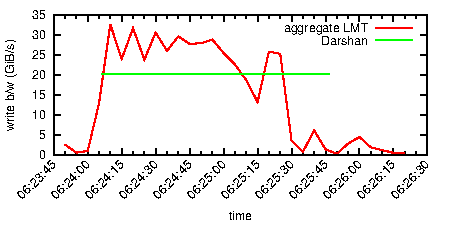
\includegraphics[width=0.5\textwidth]{figs/2k-lustre-wr-bw.pdf}
\caption{Correlating Darshan observed write interval and B/W with LMT's aggregate
write B/W for 2K VPIC run.}
\label{fig:2k-write}
\end{figure}

\begin{figure}
\centering
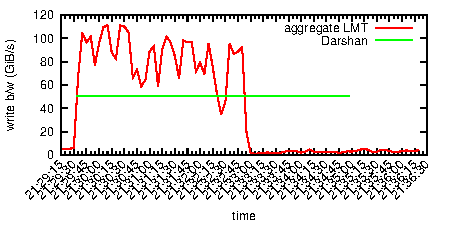
\includegraphics[width=0.5\textwidth]{figs/16k-lustre-wr-bw.pdf}
\caption{Correlating Darshan observed write interval and B/W with LMT's aggregate
write B/W for 16K VPIC run.}
\label{fig:16k-write}
\end{figure}

\section{Conclusions}

We know a little more about I/O.

\bibliographystyle{IEEEtran}
\bibliography{REFERENCES}

\end{document}
